% --------------------
\chapter{Planning}
% --------------------

\section{Introduction(ps)}
This part will describe the task that has been spliting into milestones which each task has to be complete step by step in order th achieve the final outcome.
The risk mangement has been planned carefully so any risk that is possible has a back up plan for it.
This section also includes work allocation of each member.
It also describes the group resources such as buget, laboratory equipment and customer's supply. 

%\end{itemize}

\section{Risk Management}

\subsection{Risks Planned}
A risk assessment was performed at the beginning of the project to make sure that the appropriate actions could be taken when confronted with a problem. 
The following table shows the risks the group has prepared for, the likelihood and 
impact of the risk which determines the priority of the risk, and the appropriate action in response to the risk.

\begin{center}
	\begin{tabular}{ | p{4cm} | p{2cm} | p{2cm} | p{5cm} | }
	\hline
	\textbf{Risk} & \textbf{Likelihood (1: Low, 5: High)} & 
	\textbf{Impact (1: Low, 5: High)} & \textbf{Action} \\ \hline
	Faulty Components & 4 & 4 & Order spares where feasible.
	Source new/replace faulty components as soon as possible otherwise. \\ \hline
	Team member becoming unavailable & 2 & 4 & At least two people per task.
	Reallocating people to different tasks as required. \\ \hline
	Team member facing difficulties & 5 & 2 & At least two people per task.
	Good team communication. Prioritise necessary tasks first. \\ \hline
	Tasks overrunning & 4 & 3 & Plan redundancies into Gantt Charts.
	Reallocate resources when necessary. Communicate between team members often. \\ \hline
	Loss of files/source code & 1 & 5 & Proper use of source control. Back up all source code. \\ \hline
	Loss of access to facilities & 1 & 4 & Work from home laboratory. 
	Buy missing components if necessary \\
	\hline
	\end{tabular}
\end{center}

\section{Work Allocation (ps)}

Working in a group has its advantages, but it also has drawbacks. The group has more man power and time, but the effectiveness of work allocation and other management skills must be achieved. Therefore, to use all the human resources as competent as possible, the developers have known about the specification of the project well. However, there are new parts to learn about this project. The following factor has been considered thoroughly before assigning task to any team members:

\begin{itemize}
\item	Availability of each member.

\item	The resource limitation
 
\item	The clarification of the task

\item   Time allowance for unexpected problems

\item	Each individual skills
\end{itemize}


\subsection*{Planned Work Allocation}
\label{sec:work_plan}
It is very essential that each member other coursework deadline and exams include in the consideration of work allocation. 
The engineer will work effectively if they got assigned  to their interest in the duty and that role clarified well. 
The work assigned to each individual is based on the posses sufficient skill and knowledge prior to the task. 
Each task has been assigned a task leader and it will have the another member set to the same task in case the task leader has problems with the work they have done.
However, the team members must have flexibility in their time in order to support others. 
In order to avoid work over run the time, the project has been set an earlier deadline so that if any unexpected problems happen, there are still a spare time to solve the problem. The specific skills that individuals want to mention are:

\begin{itemize}
\item Andy: Power, PCB, Control, MATLAB
\item Mitch: Image Processing, MATLAB, ASM, Report Writing
\item John: MATLAB, Image Processing, Control, Radio Transmission
\item Peak: Digital Control, Display, MATLAB, Information Theory
\item Michael: Programming, $\mu$Processors, Interfaces
\end{itemize}

Tasks have been located to each person according to this list.
The time line of the task is also important because some task for each individual depend on a completion of another task. 
This cause problems when one task got stuck and so the productiveness of the time management will be reduced. 
This can be solved by assigning another task that is not dependant on the other tasks. 

A Resource limitation is one of the factor that limited the group member to do tasks. This is because the customer provide only a single UAV and also only one camera has been purchased, so only one person can work on this device at a time. We solved this problem by having a laboratory space that the UAV will be placed their all the time so any of the team member can access it. To mange the limited resource, the only time that the individual access the UAV is when he wants to test the system. 

To clarify the tasks so the individuals can understand and also to ensure that all the tasks have been assigned to at least one member of the group is essential. 
The project will be a bottom-up design. 
Figure\ref{task allocation} shows a diagram of task allocation to each member of the group. 
The task allocation based on the task locate on the block diagram in figure\ref{fig:block1}.
The blue box between members are the task shared between the members on it's side. 
If the blue box stand on its own it means only one person is assigned to that task.

\begin{figure}[H]
\begin{center}
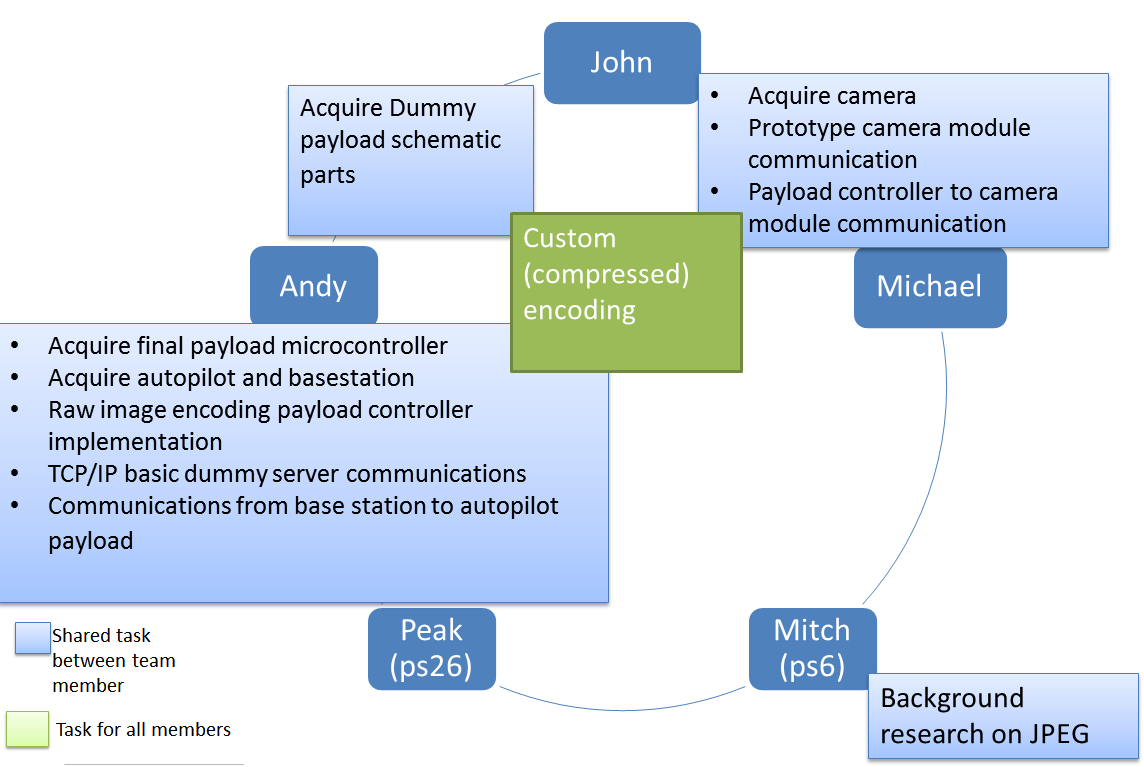
\includegraphics[width=1.0\textwidth]{figures/initial_task_allocation.png} 
\end{center}
\caption{Initial task allocation of the project\label{task allocation}}
\end{figure}

\subsubsection{Schedule - (jc)}
Considerable thought was also given to the scheduling of the tasks, an initial gantt chart was drawn up
at the beginning of the project (see appendix \ref{appendix:gantt}) with a breakdown of the tasks as we
imagined them at the start of the project.

During our regular meetings this gannt chart was used as a gauge for our progress and was ammended when
needed (i.e. our initial timing turned out to be slightly optimistic).


\section{Team resources (jc)}
\label{sec:team_resources}

This section of the management chapter covers how we controlled our use of physical resources rather than time or personnel resources. This consists of managing our budget and what we had to buy as well as what resources we had already or were provided with.

\subsection{Budget (jc)}

Our overall budget was \pounds 200 and we stayed within that while at the same time not letting it constrain us when we needed to purchase components.

\begin{table}[H]
\begin{tabular}{| l | r || r |}
\hline
\textbf{Component description} & \textbf{Quantity} & \textbf{Combined cost} \\ \hline \hline
RS485 bus transceiver (SOIC14) & 3 & 9.684 \\ \hline
RS485 bus transceiver (DIP14) & 3 & 9.756 \\ \hline
RS485 bus transceiver & 1 & 6.96 \\ \hline
Logic level converter (SOT235) & 3 & 9.684 \\ \hline
RJ45 Socket & 4 & 3.072 \\ \hline
4M flash chip (8DIP) & 4 & 2.592 \\ \hline
Arduino mega protoshield & 1 & 5.46 \\ \hline
Arduino uno protoshield & 1 & 4.38 \\ \hline
microSD breakout board & 1 & 5.99 \\ \hline
Camera module - serial JPEG TTL & 3 & 132 \\ \hline \hline
 & Total cost: & 189.58 \\ \hline
\end{tabular}
\caption{Table of expenditures}
\label{expenditure}
\end{table}

The above table (table \ref{expenditure}) details the way that the project budget was spent. The first column is a brief description of the component, the second column is the number that have been ordered and the third column is the total cost of those components.

The biggest drain on the budget was the camera modules as at \pounds 44 each these were the most expensive components. The first camera breaking was a set-back and some alternative camera options were investigated quickly but it was decided that the uCam was the best option and a new one was ordered, thankfully there was still plenty left of the budget to accommodate this.

\subsection{Electronic Material (jc)}

\subsubsection{Laboratory Equipment}

We were given access to the "Advanced Electronics Lab" on level 3 of the Zepler building. This gave us some bench-space and access to a wide range of lab equipment.

Of the lab equipment available to us the only pieces we actually used were the digital oscilloscope and the bench-top power supply. The oscilloscope was used at various stages through development to verify signals were doing what they should be, where they should be. The power supply was used to power the camera when it was discovered that the combination of SD-card and camera was drawing more current than could be supplied by the arduino.

\subsubsection{From the customer}

We were provided with a skycircuits autopilot \cite{SkyCircuits} as described in \ref{sec:autopilot_research} and some software to interface with it from the ground.

We were also provided with some example microcontroller code and a schematic for a dummy payload module i.e. a payload module that can recognise transmit tokens but that doesn't actually do anything.

\subsubsection{From ourselves}

We also had access to a range of equipment that we owned personally this included a selection of development boards:

\begin{itemize}
	\item Arduino uno, see section \ref{arduino_imp} \cite{arduino_serial_library}
	\item Olimexino-STM32 \cite{olimexino}
	\item mbed LPC1768 Header Board \cite{mbed}
\end{itemize}

This gave us a range of possibilities for investigation into different implementations and initial development.

Another bit of personally owned equipment that proved useful during development and testing was a USB to serial cable which was used to initially test the second camera with the 4D systems software \cite{ucam_test_software}, see section \ref{sec:existing_software_test}. This cable was also then used to attach the debug line for the rest of the development on the arduino platform.

The last bit of personally owned equipment that was used in this project was a micro SD card which was used for storing the images that come off the camera (see section \ref{sec:SD_imp}). The mounting for this used during development was loaned from ECS stores, this was replaced during later stages of development.

\section{Group Communication (ab) (ms)}
\label{group_comms}

\subsection{Formal Meetings}
\label{formal meetings}
For the duration of the project, we held weekly meetings on most Tuesday 
Afternoons from 4pm onwards in the Hartley Library. This would allow us to 
review progress made against progress expected, and to modify our project 
plan and allocation of work for the following week.

Minutes of these meetings would be stored in our repository.
The timing of these meetings (the afternoon before our weekly meetings with our 
supervisor) will allow us to present a clear outline 
of new developments and our week-by-week plans to our supervisor.
The meetings with our supervisor will allow the group members to assess their situation
and re-organize themselves if necessary.

\subsection{Methods of Communication (ms)}

The group was prepared to use two primary methods of communication during the project
in-between group meetings. This would allow the group to share any urgent information
with each other easily.
These methods of communication are discussed below:

\subsubsection{E-mail}

Email would be the primary form of communication between group members
in between the weekly group meetings. It will be the responsibility of each group
member to regularly check their e-mail and keep up to date with the latest 
developments of the project. Information which is useful for all members of the 
project or not directed at a specific individual would be sent by e-mail. E-mail also 
has the advantage of communicating software directly between members and leaving
an audit trail to keep track of the project's progress.

\subsubsection{Telephone}

Each group member's contact phone numbers were shared at the beginning of the
project to complement e-mail communications. A contact by phone number would
be useful if very urgent information needs to be communicated immediately between
project members. Although e-mail communication should suffice, telephone 
communication would be used to instantly contact a group member who may not
be keeping up with e-mail exchanges.

\subsection{Source Control}
\label{source control}
We decided to use version control software throughout the project, to manage 
everything from minutes to source code and payload schematics. As well as 
being a very useful tool to facilitate group work, it also helps us to meet 
our customer's request to deliver this as an open source project - at the end 
of the project, a repository could easily be gardened and presented, with the 
addition of appropriate open-source licenses at the end of the project.

Initially, we used a central Subversion (SVN) repository hosted on ECS' 
UGForge service. It was decided to use this as most of the group had 
experience using SVN. This worked well for most of the project, but 
unfortunately, something was committed to this repository that could not be 
open sourced (the customer's Ground Control Station software). This presented 
us with a problem, as although it would be trivial to revert this commit with 
the "\$ svn merge" command, this creates a new commit, and the file in 
question would remain in the repository's history and could still be accessed.

In theory, it would be possible to remove this commit from SVN history by 
using the "\$ svnadmin dump" command, filtering the offending commit out of 
the dumpfile, and regenerate the repository with the "\$ svnadmin load" 
command. However, in practice, this was not possible as our repository 
contains binary information above 64kB, therefore the ASCII editor used to 
modify the dumpfile would cut off data in the binary file after the 64kB 
limit, rendering any following data useless.

It would be possible to start a new SVN repository and check in our 
repository up to but not including the offending commit, but we would lose 
all metadata (i.e. committer, commit time, etc.). Therefore, it was decided to 
switch to git, a distributed version control system (which would allow us to 
modify project history). Converting the repository using git-svn was a trivial 
process. Although not all of the group was confident using this tool, git 
lets a committer commit on behalf of another user. Moving to git also 
allowed us to use github, a hosting service, which is free to open-source 
projects (such as ours), which also provides us with some additional 
project statistics. ??? Reference ???? Appendix ???
